\documentclass{article}

\usepackage{graphicx}
\usepackage{tikz}
\usepackage{tikzsymbols}
\usetikzlibrary{calc,patterns,shapes.geometric}
\pagestyle{empty}
\usepackage[margin=0pt]{geometry}
\geometry{papersize={14in,12in}}

\def\centerarc[#1](#2)(#3:#4:#5){\draw[#1] ($(#2)+({#5*cos(#3)},{#5*sin(#3)})$) arc (#3:#4:#5);}

\begin{document}
	\begin{figure}
		\centering
		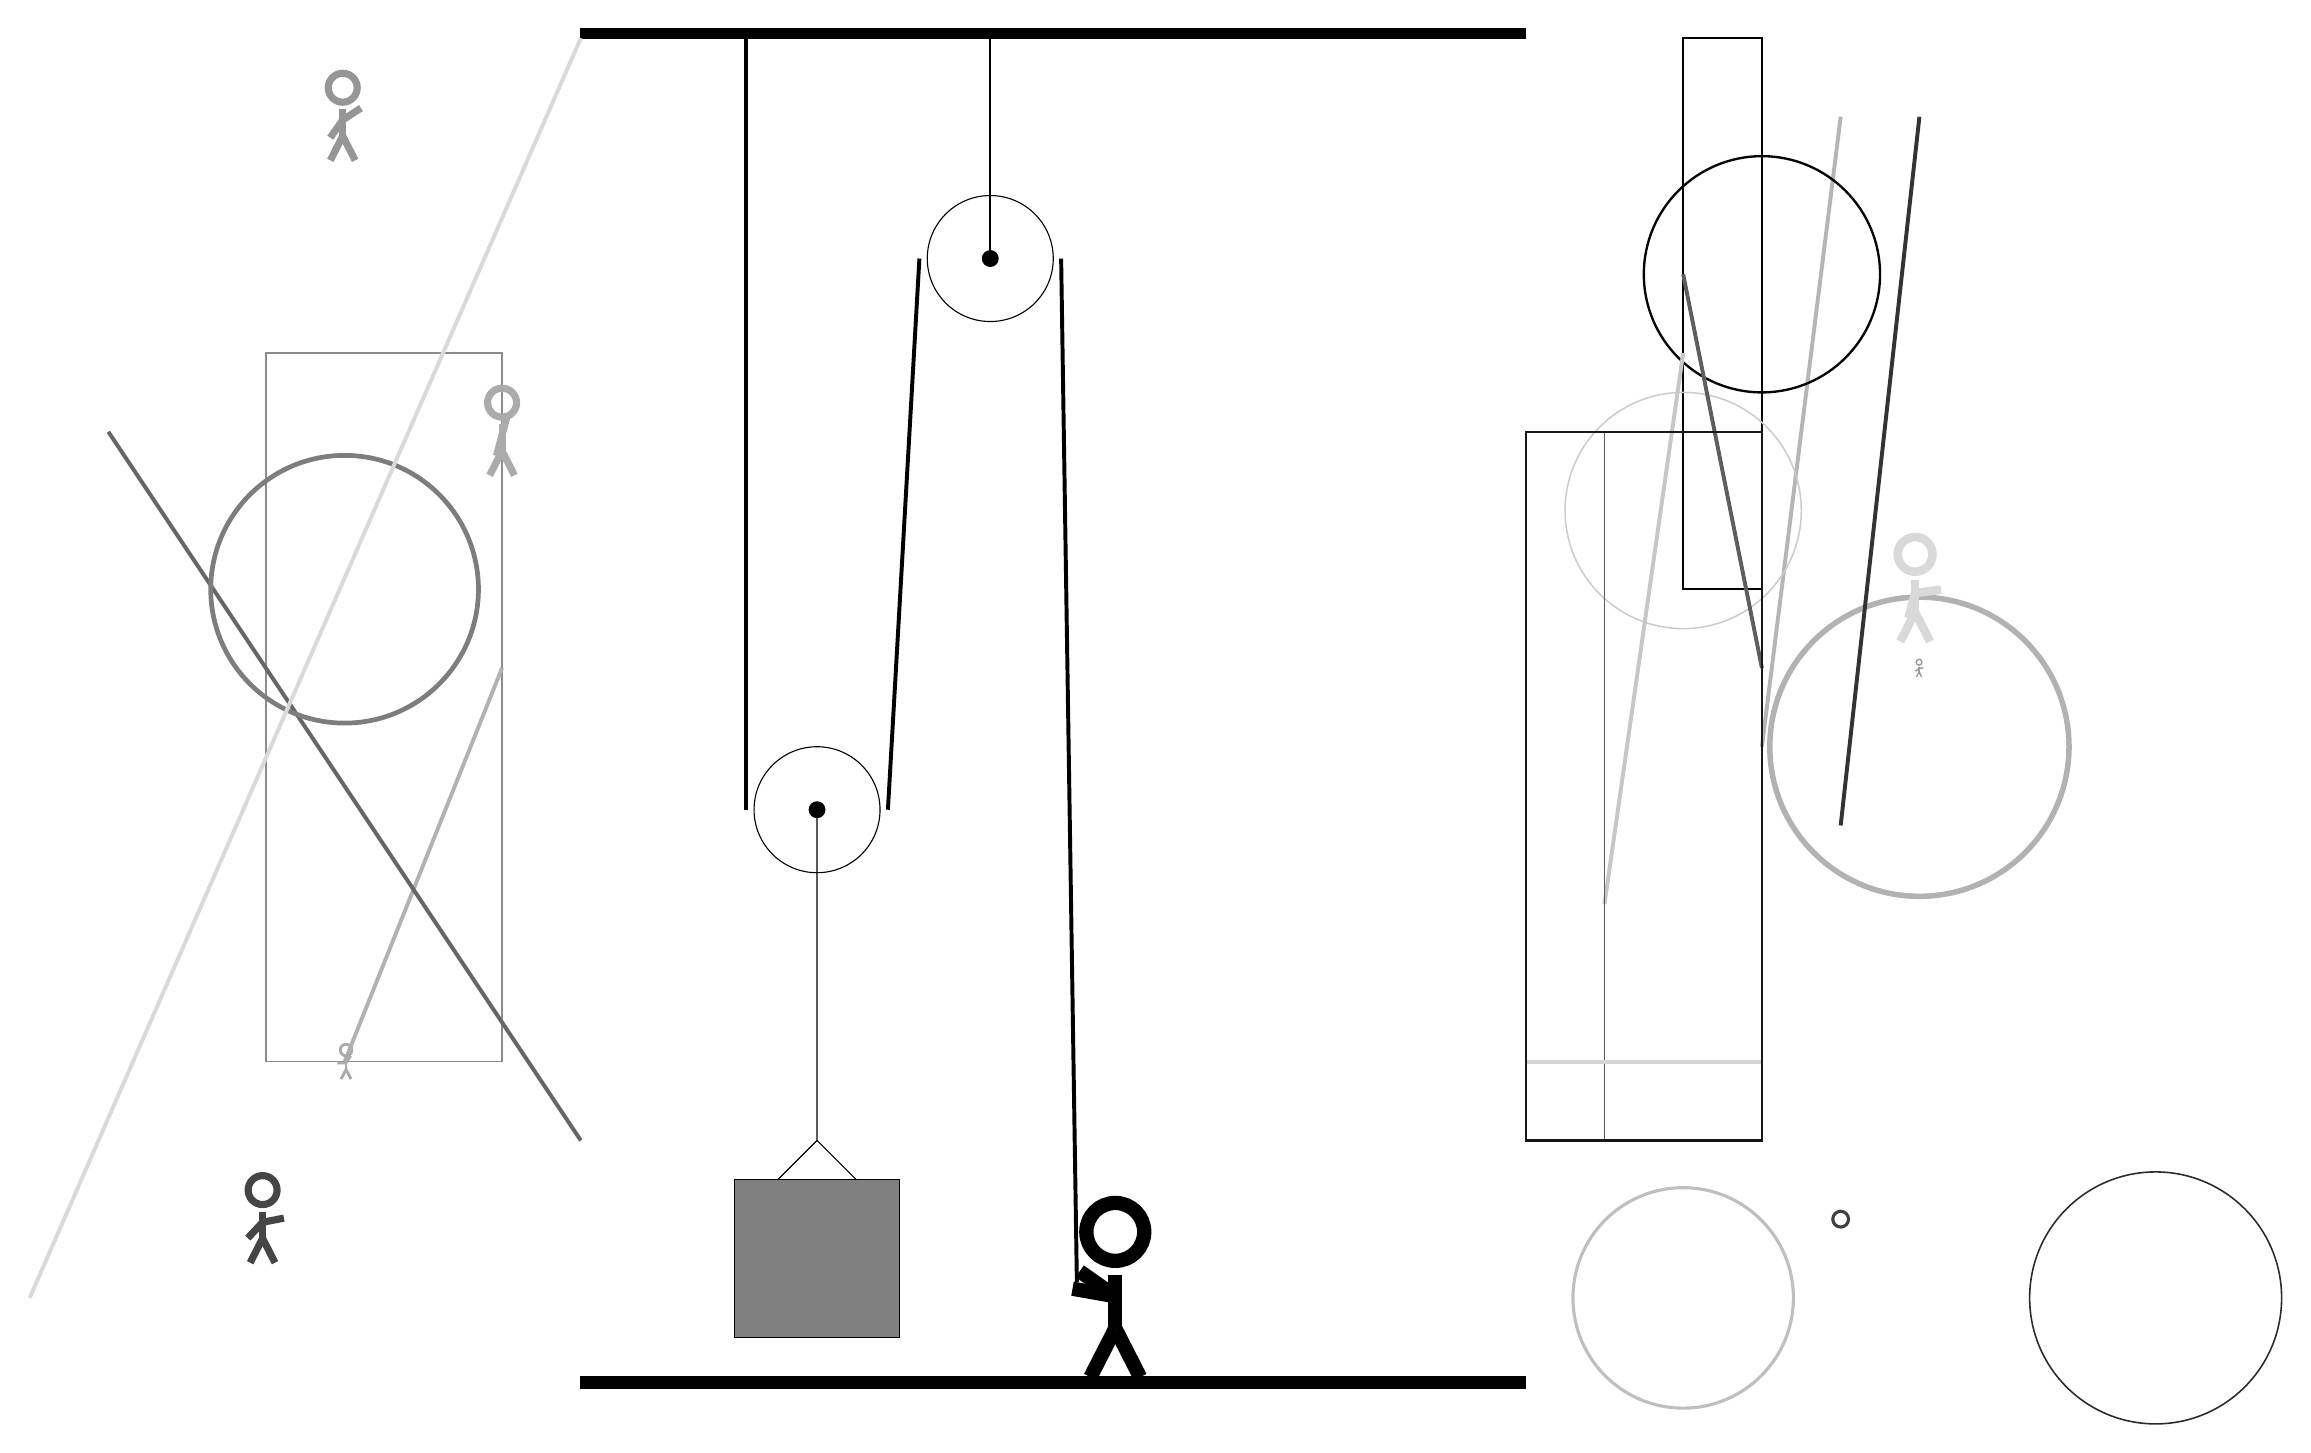
\begin{tikzpicture}
			%%%%% START %%%%%
			
			\draw[fill=black] (-2, 14) rectangle (10, 14.125);
			
			\draw (3.2, 11.2) circle (0.8);
			\draw[fill=black] (3.2, 11.2) circle (0.1);
			\draw[thick] (3.2, 11.2) -- (3.2, 14);
			
			\draw[line width=0.5mm, color=black!29](14, 13) -- (13, 5);
			
			\draw[line width=0.2mm, color=black!45] (-3, 10) rectangle (-6, 1);
			\draw[line width=0.3mm, color=black!99] (12, 14) rectangle (13, 7);
			\draw [line width=0.2mm, color=black!20](12, 8) circle (1.5);
			\draw[line width=0.5mm, color=black!30](-3, 6) -- (-5, 1);
			\draw [line width=0.7mm, color=black!30](15, 5) circle (1.9);
			\draw [line width=0.3mm, color=black!98](13, 11) circle (1.5);
			\draw[line width=0.5mm, color=black!22](11, 3) -- (12, 10);
			\node[line width=0.4mm, color=black!41] at (-5, 13) {\Strichmaxerl[5][55][33]};
			\draw [line width=0.4mm, color=black!25](12, -2) circle (1.4);
			\node[line width=0.3mm, color=black!33] at (-3, 9) {\Strichmaxerl[5][75][75]};
			
			\draw [line width=0.2mm, color=black!77](15, 8) circle (0.0);
			\draw [line width=0.4mm, color=black!75](14, -1) circle (0.1);
			
			\node[line width=0.4mm, color=black!40] at (15, 6) {\Strichmaxerl[1][35][10]};
			\draw [line width=0.2mm, color=black!83](18, -2) circle (1.6);
			\draw[line width=0.2mm, color=black!64] (10, 9) rectangle (11, 0);
			
			\node[line width=0.3mm, color=black!73] at (-6, -1) {\Strichmaxerl[5][47][11]};
			\draw[line width=0.5mm, color=black!17](13, 1) -- (10, 1);
			\draw[line width=0.5mm, color=black!63](12, 11) -- (13, 6);
			\draw[line width=0.5mm, color=black!60](-2, 0) -- (-8, 9);
			\draw [line width=0.6mm, color=black!51](-5, 7) circle (1.7);
			
			\draw[line width=0.3mm, color=black!73] (-4, 1) rectangle (-4, 1);
			\draw[line width=0.5mm, color=black!80](14, 4) -- (15, 13);
			\draw[line width=0.5mm, color=black!15](-2, 14) -- (-9, -2);
			\draw[line width=0.3mm, color=black!91] (10, 0) rectangle (13, 9);
			
			\node[line width=0.3mm, color=black!15] at (15, 7) {\Strichmaxerl[6][75][7]};
			\node[line width=0.6mm, color=black!33] at (-5, 1) {\Strichmaxerl[2][1][58]};
			
			\draw (1, 4.2) circle (0.8);
			\draw[fill=black] (1, 4.2) circle (0.1);
			
			\draw (1, 4.2) -- (1, 0) -- (0.5, -0.5);
			\draw (1, 0) -- (1.5, -0.5);
			\draw[fill=black!50] (-0.05, -0.5) rectangle (2.05, -2.5);
			
			\draw[line width=0.5mm] (0.1, 14) -- (0.1, 4.2);
			\centerarc[line width=0.5mm](1, 4.2)(180:360:0.9);
			\draw[line width=0.5mm](1.9, 4.2) -- (2.3, 11.2);
			\centerarc[line width=0.5mm](3.2, 11.2)(0:180:0.9);
			\draw[line width=0.5mm](4.1, 11.2) -- (4.3, -1.8);
			
			\node at (4.7, -1.9) {\Strichmaxerl[10][-35][170]};
			
			\draw[fill=black] (-2, -3) rectangle (10, -3.15);
			
			%%%%% END %%%%%
		\end{tikzpicture}
	\end{figure}	
\end{document}